\documentclass[11pt,a4paper]{article}

\usepackage[utf8]{inputenc}
\usepackage[english]{babel}
\usepackage{amsmath}
\usepackage{amssymb}
\usepackage{amsthm}
\usepackage{geometry}
\usepackage{listings}
\usepackage{xcolor}
\usepackage{hyperref}
\usepackage{graphicx}
\usepackage{tikz}
\usetikzlibrary{shapes,arrows,positioning,fit}

\geometry{margin=1in}

\hypersetup{
    colorlinks=true,
    linkcolor=blue,
    filecolor=magenta,      
    urlcolor=cyan,
    pdftitle={Hexaly Model: Structure, Flow, and Usage},
    pdfpagemode=FullScreen,
}

\lstdefinestyle{pythoncode}{
    language=Python,
    basicstyle=\ttfamily\small,
    keywordstyle=\color{blue}\bfseries,
    commentstyle=\color{gray}\itshape,
    stringstyle=\color{red},
    numbers=left,
    numberstyle=\tiny\color{gray},
    stepnumber=1,
    numbersep=8pt,
    backgroundcolor=\color{white},
    showspaces=false,
    showstringspaces=false,
    showtabs=false,
    frame=single,
    tabsize=2,
    captionpos=b,
    breaklines=true,
    breakatwhitespace=false,
    escapeinside={\%*}{*)},
}

\title{\textbf{Hexaly Model: Structure, Flow, and Usage}}
\author{Allocation Optimization System v2}
\date{\today}

\begin{document}

\maketitle

\begin{abstract}
This document provides a comprehensive overview of the Hexaly-based optimization model used in the allocation system. It describes the model architecture, data flow, constraint management, and operational usage patterns for the three primary optimization modes: allocation-only, scheduling-only, and integrated optimization.
\end{abstract}

\tableofcontents
\newpage

\section{Model Overview}

The unified optimizer supports three distinct operating modes, each designed to address specific fleet optimization challenges.

\subsection{Operating Modes}

\begin{itemize}
    \item \textbf{allocation\_only}: Assigns routes to vehicles, optimizing for coverage and vehicle utilization while respecting turnaround times and shift constraints.
    
    \item \textbf{scheduling\_only}: Optimizes charging schedules for vehicles with pre-determined route duties, minimizing electricity costs while ensuring energy requirements are met.
    
    \item \textbf{integrated}: Performs joint optimization of allocation and charging in a single weighted objective function, enabling coordination between route assignment and energy management decisions.
\end{itemize}

\subsection{Primary Implementation Files}

The core implementation spans three main modules:

\begin{itemize}
    \item \texttt{src/optimizer/unified\_optimizer.py} --- Main optimization model
    \item \texttt{src/optimizer/cost\_matrix.py} --- Pairwise data preparation
    \item \texttt{src/controllers/unified\_controller.py} --- Orchestration layer
\end{itemize}

\section{Architecture}

\subsection{System Flow}

The optimization system follows a structured data flow from controller to optimizer to Hexaly solver:

\begin{figure}[h]
\centering
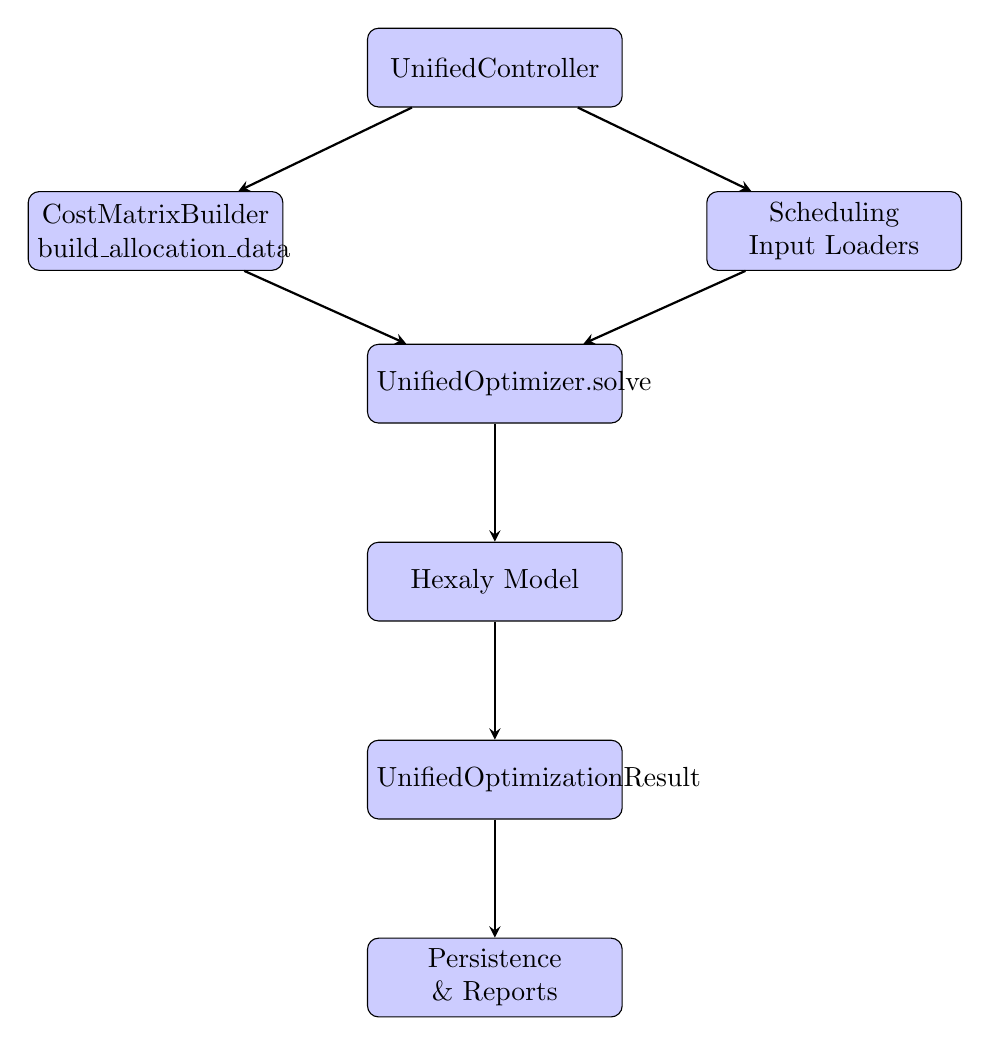
\begin{tikzpicture}[
    node distance=1.5cm,
    block/.style={rectangle, draw, fill=blue!20, text width=3cm, text centered, rounded corners, minimum height=1cm},
    arrow/.style={thick,->,>=stealth}
]
    \node [block] (controller) {UnifiedController};
    \node [block, below left=of controller] (dp) {CostMatrixBuilder\\build\_allocation\_data};
    \node [block, below right=of controller] (si) {Scheduling Input Loaders};
    \node [block, below=3cm of controller] (uo) {UnifiedOptimizer.solve};
    \node [block, below=of uo] (hm) {Hexaly Model};
    \node [block, below=of hm] (res) {UnifiedOptimizationResult};
    \node [block, below=of res] (db) {Persistence \& Reports};
    
    \draw [arrow] (controller) -- (dp);
    \draw [arrow] (controller) -- (si);
    \draw [arrow] (dp) -- (uo);
    \draw [arrow] (si) -- (uo);
    \draw [arrow] (uo) -- (hm);
    \draw [arrow] (hm) -- (res);
    \draw [arrow] (res) -- (db);
\end{tikzpicture}
\caption{High-level architecture and data flow}
\end{figure}

\subsection{Core Design Principles}

\begin{enumerate}
    \item \textbf{Native List Variables}: Allocation uses Hexaly's native list variables (\texttt{m.list}) instead of pre-generated route combinations, enabling the solver to explore assignment sequences efficiently.
    
    \item \textbf{Partition Constraints}: Route assignment uses \texttt{m.partition(routes\_by\_vehicle)} to ensure each route is assigned exactly once across all vehicles when routes exist.
    
    \item \textbf{Hybrid Constraint Management}: ConstraintManager provides pairwise feasibility and scoring (\texttt{feasible\_vr}, \texttt{score\_vr}), while sequence-level constraints (turnaround time, shift span) are enforced directly via Hexaly expressions.
\end{enumerate}

\section{Input Data Contract}

\subsection{Allocation Data Structure}

The \texttt{CostMatrixBuilder.build\_allocation\_data()} method prepares the following data structures for list-based allocation:

\begin{itemize}
    \item \textbf{score\_vr} ($n_{\text{vehicles}} \times n_{\text{routes}}$): Pairwise score matrix for vehicle-route assignments. Higher scores indicate better matches.
    
    \item \textbf{feasible\_vr} ($n_{\text{vehicles}} \times n_{\text{routes}}$): Boolean feasibility mask. Entry $(v,r)$ is 1 if vehicle $v$ can serve route $r$, 0 otherwise.
    
    \item \textbf{route\_start\_times} ($n_{\text{routes}}$): Start time for each route in minutes from optimization window start.
    
    \item \textbf{route\_end\_times} ($n_{\text{routes}}$): End time for each route in minutes.
    
    \item \textbf{route\_durations} ($n_{\text{routes}}$): Duration of each route in minutes.
    
    \item \textbf{route\_energy\_required} ($n_{\text{vehicles}} \times n_{\text{routes}}$): Energy consumption in kWh for each vehicle-route pair.
    
    \item \textbf{metadata}: Dictionary containing allocation parameters such as:
    \begin{itemize}
        \item \texttt{strict\_turnaround}: Minimum turnaround time between consecutive routes
        \item \texttt{shift\_limit}: Maximum shift duration per vehicle
        \item \texttt{preferred\_turnaround\_penalties}: Soft constraint weights
        \item \texttt{max\_routes}: Maximum routes per vehicle
    \end{itemize}
\end{itemize}

These data structures are passed directly to \texttt{UnifiedOptimizer.solve(...)}.

\section{Model Structure by Mode}

\subsection{Allocation-Only Mode}

\subsubsection{Decision Variables}

\begin{equation}
\text{routes\_by\_vehicle} = \left[ m.\text{list}(n_{\text{routes}}) \mid v \in \text{vehicles} \right]
\end{equation}

Subject to partition constraint when routes exist:
\begin{equation}
m.\text{partition}(\text{routes\_by\_vehicle})
\end{equation}

\subsubsection{Hard Constraints}

\begin{enumerate}
    \item \textbf{Route Count Limit}: Per-vehicle maximum routes
    \begin{equation}
    \text{count}(\text{list}_v) \leq \text{max\_routes\_per\_vehicle} \quad \forall v
    \end{equation}
    
    \item \textbf{Infeasible Assignment Prohibition}:
    \begin{equation}
    m.\text{contains}(\text{list}_v, r) = 0 \quad \text{if } \text{feasible\_vr}[v,r] = 0
    \end{equation}
    
    \item \textbf{Strict Turnaround}: Between consecutive routes in assignment sequence
    \begin{equation}
    t_{\text{start}}^{r_{i+1}} - t_{\text{end}}^{r_i} \geq \Delta t_{\text{turnaround}} \quad \forall \text{ consecutive } r_i, r_{i+1}
    \end{equation}
    
    \item \textbf{Shift Duration Cap}:
    \begin{equation}
    t_{\text{end}}^{\text{last}} - t_{\text{start}}^{\text{first}} \leq T_{\text{shift\_max}}
    \end{equation}
\end{enumerate}

\subsubsection{Objective Function}

\begin{equation}
\max \quad w_{\text{count}} \cdot \sum_v |\text{list}_v| + \sum_{v,r} \text{score\_vr}[v,r] \cdot \mathbb{1}_{r \in \text{list}_v} + \text{soft\_turnaround\_terms}
\end{equation}

\subsubsection{Output Extraction}

Route index collections are read from the solver solution and reconstructed as tuples:
\begin{equation}
(\text{vehicle\_id}, \text{route\_sequence}, \text{sequence\_score})
\end{equation}

\subsection{Scheduling-Only Mode}

Uses interval-based scheduling with Hexaly's native interval variables for charging sessions.

\subsubsection{Components}

\begin{itemize}
    \item Charging interval decision variables
    \item Site capacity constraints
    \item Route energy requirement checkpoints
    \item Optional charger power-class allocation
\end{itemize}

\subsubsection{Objective}

\begin{equation}
\min \quad \text{charging\_cost} + \lambda_{\text{SOC}} \cdot \text{SOC\_shortfall} + \lambda_{\text{makespan}} \cdot \text{makespan}
\end{equation}

where the makespan term is optional.

\subsection{Integrated Mode}

Combines allocation and scheduling into a unified optimization problem.

\subsubsection{Model Components}

\begin{itemize}
    \item List-based allocation decision variables
    \item Interval-based scheduling decision variables
    \item Optional route execution intervals linked to list membership:
    \begin{equation}
    \text{if\_present}(\text{route\_interval}_r) = \text{contains}(\text{route\_list}_v, r)
    \end{equation}
    \item No-overlap constraints between charging and route execution intervals
\end{itemize}

\subsubsection{Weighted Objective}

\begin{equation}
\max \quad w_{\text{alloc}} \cdot f_{\text{allocation}} - w_{\text{sched}} \cdot f_{\text{scheduling}}
\end{equation}

where:
\begin{itemize}
    \item $f_{\text{allocation}}$ is the allocation objective (route coverage + scores)
    \item $f_{\text{scheduling}}$ is the scheduling cost (electricity + penalties)
    \item $w_{\text{alloc}}, w_{\text{sched}}$ are user-configurable weights
\end{itemize}

\section{Constraint Ownership}

The constraint system uses a hybrid approach, splitting responsibilities between preprocessing and solver-level enforcement.

\subsection{ConstraintManager-Driven Constraints}

These are evaluated at the pairwise level during data preparation and encoded in the input matrices:

\begin{itemize}
    \item \textbf{Energy Feasibility}: Hard constraint, enforced via \texttt{feasible\_vr} gate
    \item \textbf{Charger Preference}: Soft contribution to \texttt{score\_vr}
    \item \textbf{Other Single-Route Constraints}: Any enabled constraints evaluated for individual routes
\end{itemize}

\subsection{Hexaly-Native Sequencing Constraints}

These are enforced directly in the optimization model:

\begin{itemize}
    \item \textbf{Strict Turnaround}: Minimum time gap between consecutive assigned routes
    \item \textbf{Preferred Turnaround}: Soft penalties for suboptimal gaps
    \item \textbf{Shift-Hours Bound}: Upper limit on total shift span across assigned routes
    \item \textbf{Partition}: Each route assigned to exactly one vehicle
    \item \textbf{Cardinality}: Maximum number of routes per vehicle
\end{itemize}

\textbf{Rationale}: This split keeps preprocessing lightweight while preserving complex sequence logic inside the solver where it can be explored efficiently.

\section{Charger Continuity by Segment}

When \texttt{charger\_allocation} is enabled, charger assignment is modeled at \textbf{segment} granularity (power class level), not as a single whole-window assignment.

\subsection{Segment Definition}

For each vehicle, segments are derived from route windows:

\begin{itemize}
    \item \textbf{pre\_first}: From optimization window start to first route start
    \item \textbf{between\_i}: From route $i$ end to route $i+1$ start
    \item \textbf{post\_last}: From last route end to optimization window end
\end{itemize}

\subsection{Continuity Rules}

\begin{enumerate}
    \item Power class assignment is \textbf{constant within} each segment
    \item Power class \textbf{may change between} consecutive segments
    \item Continuity is enforced using segment intervals with segment class choice variables
\end{enumerate}

\subsection{Capacity Semantics}

At any time $t$ or slot $s$:
\begin{equation}
\sum_{v : \text{class}_v(t) = c} \mathbb{1}_{\text{charging}}(v,t) \leq N_{\text{chargers}}^c
\end{equation}

where $N_{\text{chargers}}^c$ is the available count for power class $c$.

Additional constraints:
\begin{itemize}
    \item Fixed current-connection pins applied at segment level
    \item Nighttime continuity requirements enforced per segment
\end{itemize}

\section{Execution Flow}

\subsection{Step-by-Step Process}

\begin{enumerate}
    \item \texttt{UnifiedController.run\_unified\_optimization(...)} determines optimization mode and configuration
    
    \item \texttt{\_prepare\_optimization\_inputs(...)} loads:
    \begin{itemize}
        \item Routes and route metadata
        \item Vehicle fleet and current states
        \item Energy forecasts and electricity price schedules
    \end{itemize}
    
    \item \texttt{CostMatrixBuilder.build\_allocation\_data()} constructs pairwise allocation matrices
    
    \item \texttt{UnifiedOptimizer.solve(...)} builds the Hexaly model for the selected mode
    
    \item \texttt{model.close()} finalizes model construction
    
    \item \texttt{optimizer.solve()} invokes the Hexaly solver
    
    \item Results are extracted to \texttt{UnifiedOptimizationResult}
    
    \item Results are converted to legacy output formats
    
    \item Final outputs are persisted to database and reports generated
\end{enumerate}

\section{Usage Patterns}

\subsection{API Usage}

The unified optimization endpoint \texttt{/optimize/unified} accepts a \texttt{mode} parameter as a flag array:

\begin{lstlisting}[style=pythoncode]
# Allocation only
{"mode": ["allocation"]}

# Scheduling only
{"mode": ["charge_scheduling"]}

# Integrated with charger allocation
{"mode": ["allocation", "charge_scheduling", "charger_allocation"]}
\end{lstlisting}

\subsection{CLI Usage}

The \texttt{unified\_main.py} script supports multi-value mode flags:

\begin{lstlisting}[language=bash]
python unified_main.py --mode allocation
python unified_main.py --mode charge_scheduling
python unified_main.py --mode allocation charge_scheduling charger_allocation
\end{lstlisting}

The CLI automatically maps these flags to the internal optimizer mode representation.

\section{Operational Notes and Guardrails}

\subsection{Solver Compatibility}

\begin{itemize}
    \item The optimizer requires Hexaly 14.0+ with interval variable support
    
    \item Greedy fallback algorithm is available for scenarios where Hexaly is disabled or encounters errors
    
    \item The greedy fallback uses legacy-compatible sequence tuples internally for consistency
\end{itemize}

\subsection{Energy Coupling}

The \texttt{route\_energy\_required} matrix is prepared for future tighter integrated SOC-path coupling. Currently, scheduling hard checks still rely on the traditional scheduling requirement inputs, but the infrastructure is in place for direct energy tracking across allocation decisions.

\section{Developer Checklist}

When modifying the optimization model, developers should adhere to the following guidelines:

\subsection{Hexaly Model Best Practices}

\begin{enumerate}
    \item \textbf{Use Array Expressions}: Keep all model lookups in Hexaly expressions via \texttt{m.array(...)} and \texttt{m.at(...)}
    
    \item \textbf{Lambda Aggregations}: For list variables, prefer lambda-based aggregations:
    \begin{lstlisting}[style=pythoncode]
m.sum(list_var, m.lambda_function(lambda i: expr[i]))
    \end{lstlisting}
    over Python loops for objective terms
    
    \item \textbf{Solution Extraction}: Extract list solutions via:
    \begin{lstlisting}[style=pythoncode]
optimizer.solution.get_collection_value(list_var)
    \end{lstlisting}
    
    \item \textbf{Backward Compatibility}: Preserve compatibility with:
    \begin{lstlisting}[style=pythoncode]
UnifiedOptimizationResult.to_allocation_result(...)
    \end{lstlisting}
    tuple format for legacy system integration
    
    \item \textbf{Code Quality}: Run compile and lint checks after modifying model expressions
\end{enumerate}

\subsection{Testing Requirements}

\begin{itemize}
    \item Test all three optimization modes independently
    \item Verify fallback behavior when Hexaly features are unavailable
    \item Validate constraint satisfaction in generated solutions
    \item Benchmark solver performance on representative problem instances
\end{itemize}

\section{Key Files Reference}

\begin{table}[h]
\centering
\begin{tabular}{|l|p{8cm}|}
\hline
\textbf{File} & \textbf{Purpose} \\
\hline
\texttt{cost\_matrix.py} & Allocation data preparation, implements \texttt{build\_allocation\_data} \\
\hline
\texttt{unified\_optimizer.py} & Model construction, solve invocation, solution extraction \\
\hline
\texttt{unified\_controller.py} & Orchestration, input assembly, result persistence \\
\hline
\texttt{unified\_optimizer\_model.tex} & Detailed mathematical formulation (complementary document) \\
\hline
\end{tabular}
\caption{Core implementation files and their responsibilities}
\end{table}

\section{Conclusion}

The Hexaly-based unified optimizer provides a flexible, efficient framework for fleet optimization across allocation, scheduling, and integrated scenarios. By leveraging Hexaly's native list variables and constraint modeling capabilities, the system can explore large solution spaces while maintaining computational tractability.

The modular architecture and clear separation of concerns between constraint preprocessing and solver-level optimization enables maintainability and extensibility for future enhancements.

\end{document}
